\documentclass[10pt, a4paper]{report}  % report depends on what Im writing
\usepackage[english,greek]{babel}
\usepackage[utf8]{inputenc}
\usepackage{graphicx}
\usepackage{amsmath}  % supports many of the math that I wil need
%\usepackage[demo]{graphicx}
\usepackage{subfig}  % to enable many images on the same row
\graphicspath{ {/} }
\newcommand{\en}{\selectlanguage{english}}  % define the short command we will use in the text
\newcommand{\gr}{\selectlanguage{greek}} 

\title{$1^o$ Εργαστήριο στα Συστήματα Ελέγχου}
\author{Ε. Κατσούπης, Α. Γιουμερτάκης, Ρ. Ελληνιτάκης, Κ. Βούλγαρης}
\date{20 Μαρτίου 2021}

\begin{document}

\maketitle

\chapter{Α Μέρος Άσκησης}
\en
\section{Matlab \grκαι \en PID Control Systems }
\gr


Με τις συναρτήσεις και τα εργαλεία που μας προσφέρει η \en Matlab\gr, μπορούμε εύκολα να μοντελοποιήσουμε και να μικρορυθμίσουμε
τα συστήματα ελέγχου μας μέσω γραφεικών απεικονίσεων και έτοιμων εργαλείων. Μερικά απο αυτά είναι το \en PID Tuner\gr, που χρησιμοποιήσαμε
για να τελειοποιήσουμε τα βάρη των συστημάτων ελέγχου μας, η συνάρτηση\en feedback()\gr που ορίζει τον βρόγχο ανάδρασης μεταξύ εξόδου και 
εισόδοι του κυκλώματος μας, της  \en pidstd()\gr που μας βοηθάει να ορίσουμε ένα \en control system\gr με τις μεταβλητές που του δίνονται κ.α.

\section{Κώδικες \en Matlab\gr}

\begin{figure}[h] 
    \centering
    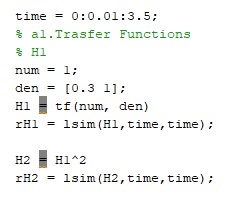
\includegraphics[width=0.4\textwidth]{1aHdefinition}
    \caption{Ο ορισμός των συναρτήσεων μεταφοράς και των αποκρίσεων τους.}
    \label{fig:define_tf}
\end{figure} 
\begin{figure}[h] 
    \centering
    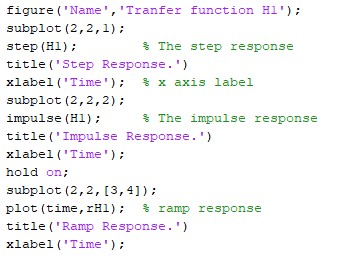
\includegraphics[width=0.5\textwidth]{1aH1}
    \caption{Δημιουργία παραθύρου προβολής της βηματικής απόκρισης του Η1.}
    \label{fig:create_plot}
\end{figure} 


Για να ορίσουμε την συνάρτηση μεταφοράς που μας δίνεται απο την εκφώνηση, και σύμφωνα με την εικόνα 1.1, χρησιμοποιούμε την μέθοδο \en \textbf{tf()} \gr της \en Matlab \gr
και της δίνουμε ώς όρισμα πίνακες για τον αριθμιτή και τον παρονομαστή, που αντιστοιχούν σε κάποια τάξη πολυωνύμου και τους συντελεστές 
της. Παρατηρούμε οτι η δεύτερη συνάρτηση μεταφοράς είναι η πρώτη αλλα υψωμένη στο τετράγωνο, οπότε δεν την ορίζουμε απο την αρχή. 


Χρησιμοποιούμε το \en \textbf{lsim()} \gr για να μπορέσουμε αργότερα να προβάλλουμε την γραφική παράσταση της απόκρισης ράμπας του κάθε
συστήματος, όπως φαίνεται στην εικόνα 1.2, και έπειτα με την χρήση της \en subplot() \gr ορίζουμε τα παράθυρα με τις γραφικές παραστάσεις, και μέσω της \en \textbf{step()} \gr παίρνουμε
την \textbf{βηματική απόκριση}. Έπειτα, για την \textbf{κρουστική απόκριση}, δίνουμε την συνάρτηση μεταφοράς μας στην μέθοδο \en \textbf{impulse()}\gr 
η οποία μας προβάλλει την γραφική απεικόνιση της κρουστικής απόκρισης στο αναδυόμενο παράθυρο. Τέλος, για την \textbf{ απόκριση ράμπας} χρησιμοποιήσαμε 
πιο πάνω όπως αναφέραμε την \en \textbf{lsim()} \gr, το αποτέλεσμα της οποίας προβάλλουμε στο παράθυρο γραφικών. Η ακριβώς αντίστοιχη διαδικασία
ακολουθήθηκε και για την δεύτερη συνάρτηση μεταφοράς.



\begin{center}
\begin{figure}
\subfloat[Η κρουστική, η βηματική και η απόκριση ράμπας του H2.]{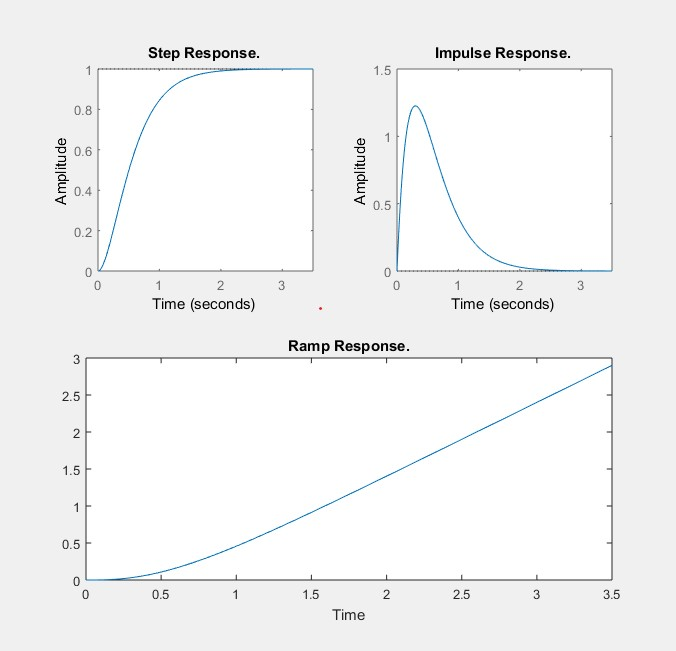
\includegraphics[width = 2.5in]{H2responses}}
\subfloat[Η κρουστική, η βηματική και η απόκριση ράμπας του H1.]{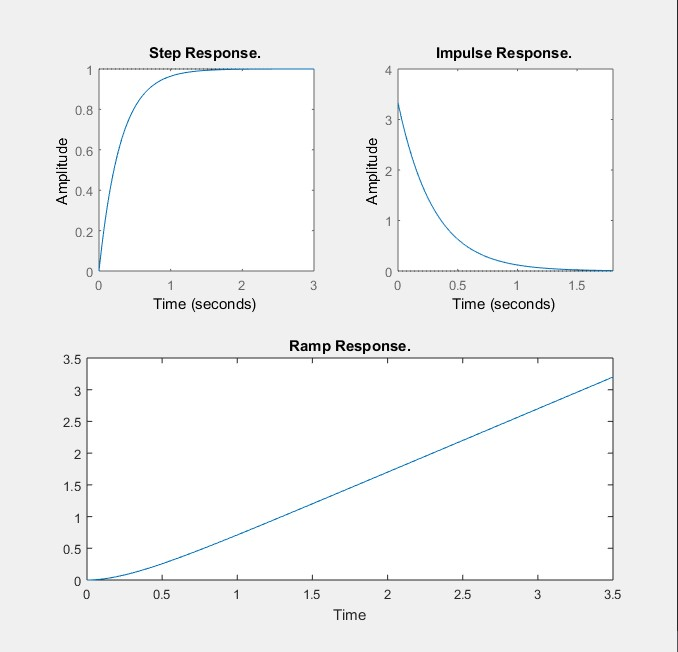
\includegraphics[width = 2.5in]{H1responses}}
\caption{}
\end{figure}
\end{center}

\section{Γραφικές Παραστάσεις}

\begin{figure}[h] 
    \centering
    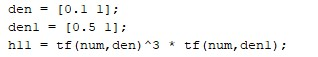
\includegraphics[width=0.6\textwidth]{1aH11}
    \caption{Ορισμός της συνάρτησης μεταφοράς H11.}
    \label{fig:definition_of_h11}
\end{figure} 

\begin{figure}[h] 
    \centering
    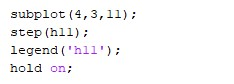
\includegraphics[width=0.5\textwidth]{1aH11plot}
    \caption{Γραφική αναπαράσταση της συνάρτησης μεταφοράς του H11.}
    \label{fig:plot_of_h11}
\end{figure}


Για τις γραφικές παραστάσεις χρησιμοποιήθηκε αντίστοιχη διαδικασία με την προαναφερθείσα στο τμήμα 1.2, με χρήση της \en \textbf{tf()} \gr για ορισμό των 
συναρτήσεων μεταφοράς, της \en \textbf{subplot()}\gr  για άνοιγμα παραθύρων πολλαπλών γραφικών και της \en \textbf{step()} \gr για αναπαράσταση της 
βηματικής απόκρισης. Ονομάσαμε τις συναρτήσεις μεταφοράς με διαδοχικά ονόματα \en \textbf{h1,h1,h3...h12}\gr για εύκολη αναγνώριση και ανάγνωση.
Για απλούστευση της διαδικασίας, όπως φαίνεται στην εικόνα 1.5 για να κατασκευάσουμε τον σύνθετο παρονομαστή, ορίζουμε δύο διαφορετικές 
συναρτήσεις και υψώνουμε και πολλαπλασιάζουμε αντίστοιχα, όπως παρακάτω:
\[ \frac{1}{0.5*s+1} \frac{1}{(0.1*s+1)^3}=\frac{1}{(0.5s+1)(0.1s+1)^3} \]
Το τελικό αποτέλεσμα αποτυπώνεται στο σχήμα 1.5.
\begin{center}
\begin{figure}[h] 
    \centering
    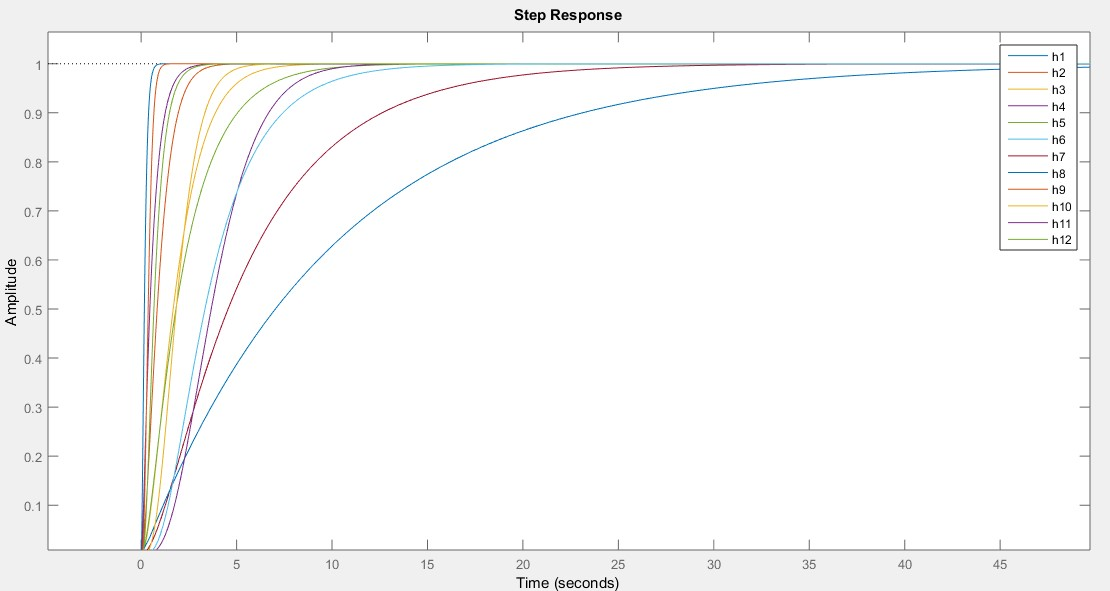
\includegraphics[width=0.9\textwidth]{h1-h12_same_plot}
    \caption{Γραφική απεικόνιση της βηματικής απόκρισης των συναρτήσεων \en h1-h12\gr.}
    \label{fig:first_all_plots}
\end{figure}
\end{center}




\chapter{B Μέρος Άσκησης}
\section{Υπολογισμός Συνάρτησης Μεταφοράς}


Για να ξεκινήσουμε την υλοποίηση του μοντέλου ελεγκτή, ορίζουμε αρχικά το σύστημα ανοικτού βρόγχου τρίτης τάξεως που μας δίνεται στην περιγραφή της άσκησης, με
όρους \en \textbf{Ks=1.0}, \textbf{$T_1$=2.0}, \textbf{$T_2$=2.0}, \textbf{$T_3$=2.0}. \gr
Απο τον ορισμό των συναρτήσεων μεταφοράς στην \en Matlab\gr , προκύπτει η συνάρτηση μεταφοράς:
\[ \frac{1}{8s^3+12s^2+6s+1}\]

\section{\en Ziegler-Nichols PID System\gr}


Χρησιμοποιώντας έναν βρόγχο \en \textbf{for}\gr με βήμα 0.5 απο το 1 έως το 20, ορίσαμε έναν \en controller P \gr και και ένα \en \textbf{feedback(sys*cont,1)}\gr    
υπολογίσαμε την γραφική παράσταση της μοναδιαίας ανάδρασης με την συνάρτηση \en \textbf{stepinfo()}\gr. Ελέγχοντας σε κάθε loop εάν το \en \textbf{peakTime == Inf}\gr 
μπορούμε να βρούμε ακριβώς σε ποιό \en Kp \gr έχουμε μόνιμες ταλαντώσεις του συστήματος, διακόπτωντας τον βρόγχο με την εντολή \en break\gr και κρατώντας την τιμή 
του \en Kcrit\gr, οπου πειραματικά υπολογίστηκε στην τιμή \textbf{8.000000}. Επίσης, μετρώντας την απόσταση μεταξύ δύο κορυφών 
στην προαναφερθείσα ταλάντωση με το \en \textbf{findpeaks()}\gr  και έπειτα χρησιμοποιώντας το
\en \textbf{max(diff())}\gr  για τον προσδιορισμό μίας μοναδικής τιμής \en Tcrit\gr, η οποία βγαίνει πειραματικά στην τιμή \textbf{7.306870}.

% Multiple images in the same line

\begin{center}
\begin{figure}
\subfloat[Απόκριση με μικρό \en Kp\gr]{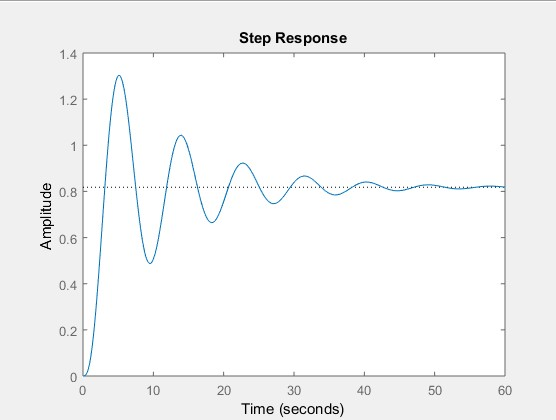
\includegraphics[width = 1.7in]{before_Kcrit2}}
\subfloat[Απόκριση \en Kp\gr  λίγο μικρότερο του \en Kcrit \gr]{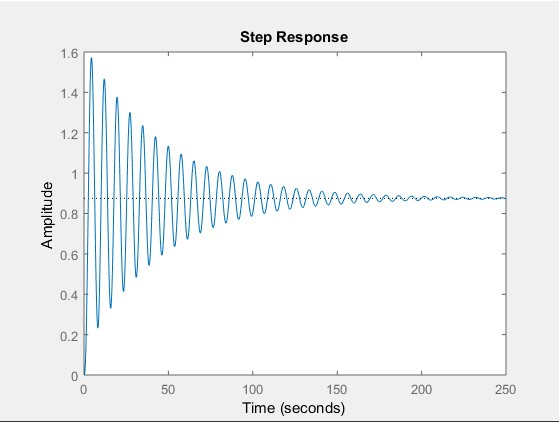
\includegraphics[width = 1.7in]{before_Kcrit1}}
\subfloat[Απόκριση με με μόνιμη ταλάντωση σε \en Kcrit \gr]{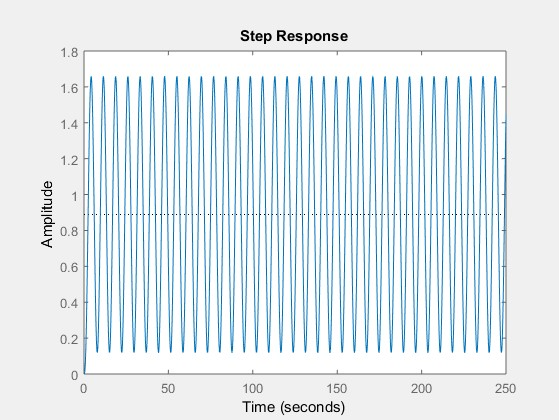
\includegraphics[width = 1.7in]{Kcrit_oscillation}}
\caption{}
\end{figure}
\end{center}






\end{document}
